%% Nemanja Milosevicr
%% phd text

%% feel free to reuse parts (or all) of the formating
%% in other words the Latex code can be used as Public Domain

%% The text itself is released under a CC-BY-SA 4.0 licence

%% Most of the code presented can be found under a GPL licence

\documentclass[b5paper]{book}

%custom packages
\usepackage[T1]{fontenc}
\usepackage[utf8]{inputenc}
\usepackage[serbian,english]{babel}

\usepackage[autostyle=true]{csquotes}
\DeclareQuoteAlias{croatian}{serbian}

% needs this declaration for ayodeji
\DeclareUnicodeCharacter{1ECD}{\d o}

%change the default font
\usepackage{lmodern}
\usepackage{nimbusmono}
\renewcommand{\familydefault}{\sfdefault}

\usepackage{ccicons}

\usepackage{ctable}
\usepackage{wrapfig}

\newcommand{\autor}{Nemanja Milošević}
\newcommand{\autorkratko}{N.-Milošević}
\newcommand{\naslov}{Negative Deep Learning}
\newcommand{\naslovsr}{Negativno duboko učenje}

\usepackage[style=authoryear-comp,sorting=nyt,maxnames=4,backend=biber,backref=true,natbib]{biblatex}

\AtEveryCite{%
  \let\parentext=\parentexttrack%
  \let\bibopenparen=\bibopenbracket%
  \let\bibcloseparen=\bibclosebracket}

\addbibresource{references.bib}

% use parens for cite

\let\oldcite\cite
\let\cite\parencite


% pdf export settings
\usepackage[%
%colorlinks,
bookmarksopen,bookmarksnumbered,citecolor=red,
%urlcolor=red,
pdffitwindow=false,unicode=true,%
pdftitle={\naslov},%
pdfauthor={\autor}%
]{hyperref}

\usepackage{graphicx}
\usepackage{fancyhdr}

\fancypagestyle{plain}{%
\fancyhead{} % get rid of headers on plain pages
\fancyfoot{}
\renewcommand{\headrulewidth}{0pt} % no lines
\renewcommand{\footrulewidth}{0pt} % 
}

% empty pages, really empty
\makeatletter
\def\cleardoublepage{\clearpage\if@twoside \ifodd\c@page\else
\hbox{}
%\vspace*{\fill}
%\begin{center}
%This page intentionally contains only this sentence.
%\end{center}
%\vspace{\fill}
\thispagestyle{empty}
\newpage
\if@twocolumn\hbox{}\newpage\fi\fi\fi}
\makeatother

% put figures in the figures folder
\graphicspath{{./figures/}}

\usepackage[figure,table,page]{totalcount}

\newcounter{citenum}
\AtEveryBibitem{\stepcounter{citenum}}

\usepackage{amsthm}
\usepackage{amsmath}
\usepackage{latexsym}

\usepackage{listings}

% if we want to make an index at the end we need this
% this document didn't have an index in the end
%\usepackage{makeidx}

%\makeindex

\lstset{
        basicstyle=\small\ttfamily,
        showstringspaces=false,
        breaklines=true
}

\lstloadlanguages{Python}

\lstnewenvironment{codeblock}
{\lstset{basicstyle=\footnotesize\ttfamily,
        columns=fixed}}
{}

%options to the lst can be given through this
\lstnewenvironment{codeblock1}[1]
{\lstset{basicstyle=\footnotesize\ttfamily,#1,
        columns=fixed}}
{}

\lstnewenvironment{codeblockw}
{\lstset{basicstyle=\footnotesize\ttfamily,
    language=wsl,
        columns=fixed}}
{}
\lstnewenvironment{codeblocka}
{\lstset{basicstyle=\footnotesize\ttfamily,
    language=[x86masm]Assembler,
        columns=fixed}}
{}
\lstdefinestyle{asmblock}{
  language=[x86masm]Assembler,
  basicstyle=\footnotesize\ttfamily
}
\lstdefinestyle{codeblock}{
        basicstyle=\footnotesize\ttfamily,
        columns=fixed,
        language=wsl
}

\lstdefinestyle{codeblockb}{
        basicstyle=\normalsize\ttfamily,
        columns=fixed,
        language=wsl
}


%% `skica' is Serbian for `sketch', these blocks were used in the development
%% of the document for various reminders

% skica can take a normal paragraph and present it more or less as such
\newcommand{\skica}[1]{
    \noindent \framebox{\parbox[c]{0.9\textwidth}{  {\small** {#1}  }}
    \newline }
}

% skicas is a small sketch, intended mostly for inline use
\newcommand{\skicas}[1]{
    \framebox{* \small \textit{#1} *}
}

% b is for bold sketches, things that are high priority
\newcommand{\skicab}[1]{
  \noindent \framebox{\parbox[c]{0.9\textwidth}{ {\small***
        \textbf{#1} }} \newline } }

% special words inline such as class and method names
%\newcommand{\kod}[1]{{\small\texttt{#1}}}
\newcommand{\kod}[1]{\lstinline[]`#1`}
\newcommand{\code}[1]{\lstinline[]`#1`}
\newcommand{\codea}[1]{\lstinline[style=asmblock]`#1`}
\newcommand{\codew}[1]{\lstinline[style=codeblock]`#1`}

%% these commands were used to get a clean version of the text
%% without the sketches

%\renewcommand{\skica}[1]{}
%\renewcommand{\skicas}[1]{}


% experimental, for one line of par being split over a page
\widowpenalty=10000
\clubpenalty=10000

% ----------------===========--------------------------------------
%                 start paper


\author{\autor}
\title{\naslov}
\date{Novi Sad, 2020}
\begin{document}
\frontmatter

\newcommand{\makemytitle}{
  \begin{center}

	
\includegraphics[width=1.8cm]{pmf-logo}\hspace{\stretch{1}}
	\parbox[b]{45ex}{\centering
          University of Novi Sad\\
Faculty of Sciences\\
Department of Mathematics and Informatics\\ }\hspace{\stretch{1}}
	
\includegraphics[width=1.8cm]{uns-logo}

	\vspace{15ex}

	\parbox[b]{\textwidth}{{\Large {\bf \hspace{0.5cm}Nemanja Milošević}}}
	\vspace{4ex}

	{\huge
            \setlength{\baselineskip}{1.5\baselineskip}\textbf{\naslov}\par}

	\vspace{4ex}
	-- Doctoral dissertation  --

        \vspace{5ex}

	{\huge
            \setlength{\baselineskip}{1.5\baselineskip}\textbf{\naslovsr}\par}

	\vspace{4ex}
	-- Doktorska disertacija  --

	\vfill

	Novi Sad, 2020
	\end{center}
	\thispagestyle{empty}
	\newpage
}

\makemytitle

~

\vfill

\thispagestyle{empty}
\noindent CC BY-SA \ccbysa\\
\textcopyright \ 2020 Nemanja Milošević\\
This work is licensed under a
Creative Commons Attribution Share Alike 4.0 International Licence
\url{https://creativecommons.org/licenses/by-sa/4.0/}

\chapter{Preface}
\chapter{Abstract}

\tableofcontents

\mainmatter

\part{Introduction}

In the first part of this dissertation a short history of the field is presented with focus on some models and approaches used later to define and describe negative deep learning models. 

\chapter{Artificial Intelligence: A brief overview}

Artificial intelligence is an universal field. Whether it is writing poetry, playing chess, proving theorems, self-driving cars or any other intellectual task, throughout history scientists have tried different artificial intelligence (AI) methods to bring the machines closer to us humans. Even though we think AI is the "new and hot" field in Computer Science, modern AI roots can be traced all the way to World War II. The name was coined after (in 1956) but the science was there long before that. From Alan Turing to Yann LeCun and others, generations have been working hard to bring the dream closer to reality -- a dream where machines can think, and reason. From the iconic Turing test to the deep neural networks, we have come long way but we still have loads to discover.

\section{History of Artificial Intelligence}

Many have tried to precisely define what AI means. Today, we know that a single, all encompassing definition is very difficult to formulate. AI is concerned with reasoning, behaviour, thought process, rational thinking and other well-defined terms. Therefore we define AI as a sum of everything that makes machines perform closely to human level. In other words machines need to learn to do the "right thing", given the knowledge we possess.

@@@ IAN
In the early days of AI, researchers sought ways to solve difficult problems for humans. These problems proved to be easy for machines to comprehend through a series of formal, mathematical rules. The real challenge today is solving the tasks that easy for humans but hard to describe formally -- problems that feel automatic, intuitive like recognizing spoken words or faces in images.

To try and provide the scientific world with an operational definition of intelligence, Alan Turing (1950) devised the famous Turing Test. A machine (in other words software) passes the test if a human asking series of questions cannon tell whether the responses are coming from a person or a computer. To develop software able to do this is not an easy task. The system would have to have many capabilities including: natural language processing (so it can communicate), knowledge representation (so it can store what it knows), automated reasoning (to draw conclusions from the knowledge) and machine learning (to adapt to new environments and detect and understand patterns in knowledge). In addition to these capabilities if we were not to avoid human-machine physical contact, the machine would also have to be able to see (computer vision) and interact with the real physical world (robotics). The six capabilities remain relevant today, 70 years after the Turing Test was formulated.

Today, researchers are not pursuing the solution to the Turing Test actively as before. The reason in in believing that it is more important to study the underlying principles of intelligence, than to duplicate it. 

With that in mind, comes the state-of-art-approach as of today -- Deep Learning.

Our "seat of consciousness", the brain, is the main object of study in neuroscience. Even though even today, the exact way in which the brain functions remains one of the great (if not the greatest) mysteries of science, the simple fact that it does enables the drive of researchers to push further and further in the quest of fully understanding the how and the why. In the 18th century, humanity was certain that the brain is the center of reason in humans, and in the 19th century we were made aware the brain contains many neurological cells called neurons. (Golgi, Broca) In the early 20th century, Nicolas Rashevsky was the first to apply mathematical models in studying the nervous system. 

Neurons or nerve cells are built from two major parts: cell body (soma) which contains a cell nucleus and a number of fibers called dendrites on of which is longer than the others (axon). Axon length is particularly interesting, some can be up to a meter long. A typical biological neuron makes connections with 10 to 100000 other neurons at junctions which are called synapses. Signals are propagated though neurons by the means of a complicated electrochemical reaction. The signals are used to control brain activity but can also enable long-term changes in connections between neurons. We believe that these mechanisms enable our brains to learn. It is amazing to think that a structure of simple cells can lead to thoughts or that in other words: brains cause minds (John Searle, 1992).

\section{Reappearance of Neural Networks with modern hardware development}

With modern GPU (graphical processor unit) development, especially the developments related to the NVIDIA CUDA framework, deep neural network models were suddenly possible and obtainable.

The human brain consists of around 100000000000 neurons (10\^11). A modern computer can have even more transistors, thus we are approaching singularity -- a point in time where computers reach superhuman levels of performance. The raw comparison is not especially informative (or right) since that even if one made a computer with unlimited resources and capabilities, we still would not know how to achieve brain's level of intelligence.

In the mid 1980s at least four different research groups revisited backpropagation learning algorithm developed 20 years earlier by Bryson and Ho. The so called connectionist model was seen by some as a direct competitor to previously developed symbolic models and also to the logicist approach. The current view is that all these approaches are complementary, not excluding.

\section{Modern Machine Learning}

As algorithms developed and we learned more and more about intelligence, one thing was very clear: AI systems must have the ability to acquire their own knowledge. This is done by extracting knowledge (patterns) from raw data. The performance of the system still relies heavily on the operator in crucial way and that is the was the data is represented. This is why almost all algorithms require specific data presented in a specific way in order to be useful. Each piece (called feature) of information can be very important. Machine learning algorithm outcome is influenced by the feature values, in other words the algorithm learns to correlate these feature values and the outcome values.

In many tasks it is very difficult to define data structures in a way that it is easy to extract meaningful feature values. This is why researchers rely on fields like representation learning where the algorithm is forced to not only provide some reasoning or outcome of the feature value inputs but also a different, more efficient representation of the input features. These representations can be very complex and difficult to interpret and that is why today we rely on stacking many simplified versions of them. If we were to draw the structure of these algorithms we would need a lot of space, because we can make them very deep. So deep in fact that they are called: Deep Learning algorithms.

\chapter{Deep Learning and its common uses}

Deep Learning uses stacked feature representations to define complex relationships between input patterns and output data. With Deep Learning, we can build complex concepts out of simpler concepts, and that is a very powerful paradigm. 

The simplest example of this concept is a multilayer perceptron (MLP). This structure is a simple mathematical function mapping a set of input values to a set of output values. However, the beauty of it is in that the complex function (MLP) is built from other simpler functions of which they are many. Every calculation of formulas applied to any data point inside a MLP can be thought as a new representation of the input data. MLP's and other similar models are often called Universal Function Approximators. 

The main idea of Deep Learning (DL) and its stacked representations of the input data provides one perspective in which we judge different DL algorithms. Another perspective comes also from depth but in slightly altered way. By using many layered representations of data we allow the machine to process data in a series of steps which is very important for some tasks and makes the algorithms learn better as they focus on smaller steps at a time. The deeper the network, the larger is the number of steps taken towards the solution. Sequential reasoning is powerful because later decisions can refer back to previous decisions. 

% TODO dodati common uses

\section{Deep Neural Networks}

We already described partly how Deep Neural Networks function in the previous section. In this section we can explain with more detail and understanding by providing a simple example.

In Figure \ref{fig:dnn_classify} we can see a simplified diagram of how a deep neural network can classify images. Other machine learning algorithm, which do not used stacked data representations often struggle with image related tasks. This is because the raw sensory input (pixel data) is not a very good representation of knowledge found in images, even though it is a good representation from a computer science standpoint. If we were to write a single function mapping pixel data to an output class representing object identity, it would be extremely complicated. Deep Learning can solve this task with ease by breaking the complexity of the mapping functions into a series of nested simpler representations, or layers. By creating a series of layers which are able to extract increasingly abstract features from an image, we create an algorithms which is able to process and distinguish between different classes of objects and successfully classify them. The input layer is sometimes also called the visible layer as it is the last data representation visible (and understandable) to us humans. Following it, there is a series of hidden layers, called hidden because their values are not given in the input data but rather calculated from the input data. In a way, they represent hidden knowledge inside the input data. The model must learn to determine which concepts from these hidden layers are useful for explaining the relationships between input and output data. In our example, and visible in the figure, every layer can detect increasingly abstract and complex structures in input data (image). The first layer given pixels detects edges, by for example comparing brightness in neighboring pixels. The second layer, given edges can detect corners and contours. The third layer given contours, and corners can detect whole sub-objects in the image by finding specific groups of given inputs (contours, edges etc.). Finally, the last layer which receives inputs of sub-objects present in an image can be used to recognize the object in a given input image.

\begin{figure}
    \centering
    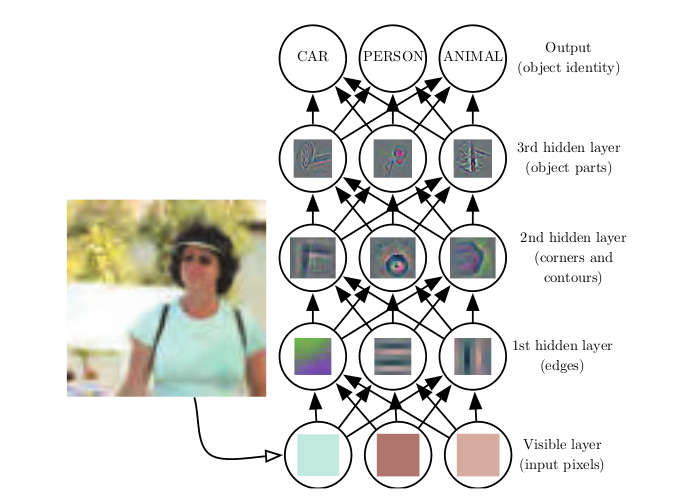
\includegraphics[scale=0.5]{figures/image-classification.png}
    \caption{Image Classification Deep Neural Network @@@IAN}
    \label{fig:dnn_classify}
\end{figure}

\section{Convolutional Neural Networks}



\subsection{Convolutional Kernels}
\section{Recurrent Neural Networks}
\subsection{Modern memory and attentive models}
\section{Image Classification Tasks}
\subsection{ImageNet}
\section{Object detection and tracking in images and videos}
\section{Natural Language Processing}
\section{Generative Models}
\subsection{Adversarial Learning}
\section{Deep Reinforcement Learning}

\chapter{Future of Deep Learning}

\section{Modern Neural Network Architectures}
\subsection{Transformers}
\subsection{Federated Learning}
\section{Towards Artificial General Intelligence}

\part{Negative Learning}

\chapter{Negative Learning}

\section{Introduction to Negative Learning}
\section{Reasoning and possible benefits of Negative Learning techniques}
\section{Policy-based algorithms and Negative Learning}
\section{Negative Learning in other algorithms}

\chapter{Negative Deep Learning}

\section{Negative Deep Learning -- Introduction}
\section{Possible Models of Negative Deep Learning}
\subsection{Missing Features}
\subsection{Partial Input Sample Training}
\subsection{Negative Output Learning}
\subsection{Ensemble Networks and upgrades of existing models}
\subsection{Agent Environments}
\section{Negative Deep Learning Use Cases}
\subsection{Object Detection and Image Classification with Occlusions}
\subsection{Neural Network Robustness}
\subsection{Neural Adversarial Attacks}
\subsection{Black-box attacks}
\subsection{White-box attacks}
\subsection{Negative Neural Networks for Regression Tasks}
\subsection{Other uses}

\part{Classification Based On Missing Features}

\chapter{Introduction}
\section{Intuition behind Missing Feature Representations}
\section{Examples of deduction with Missing Features Classification}

\chapter{Motivation}
\section{Robustness of Image Classifiers}
\section{Partial Input Classification}

\chapter{Implementation}

\section{The Negative Function}
\subsection{Activation Function Experiments}
\subsection{Negative Convolutional Kernel Experiments}
\subsection{Influence of the Negative Function in forward and backward passes}
\subsection{Influence of multiple-step training}
\subsection{Negative feature selection process}
\subsubsection{Detecting relevant features per-class for negation}

\section{Training process}

In this section training processes related to the negative learning method are described with the focus on two very important processes: multiple phase training and convolutional kernel freezing. To successfully implement the classification based on missing features model our experiments have shown that both of these techniques have to be used.

\subsection{Multi-phase training}

During the Negative Deep Learning model/hypothesis testing one interesting concept was used -- multi-phase training. Multiple phase training is a training process where after a number of training epochs some layers are frozen and reused and some of the layers are reset. In a way, multiple phase training is a regularization technique similar to Dropout with P=1.0 where some layers are completely destroyed and retrained during training. 

In our concrete example multiple phase training was used to extract and reuse convolutional layers from an image classification model. After a number of epochs all the convolutional kernels were extracted and used in other (negative) models.

\subsection{Convolutional Kernel Freezing}

For most of here mentioned models we use freezing of convolutional kernels. Freezing is a process of setting convolutional layers as fixed, constant values after they have been learned. The freezing of the convolutional layers is important from the analysis standpoint as we want to test our model modifications which are currently after the convolutional blocks. If we were not to freeze the convolutional layers, they would change their parameters during training -- and this is not desired behaviour. 

Freezing of the layers is a procedural process where one has to iterate through convolutional filter parameters (conv. kernels) and mark them as constant. In the PyTorch framework this is done with the "required\_grad" field.

Freezing of the convolutional layers (or other parts of a neural network models) is a common technique when using pre-trained models. The idea behind pre-trained models is simple: a model trained on a dataset (usually large, not easy to retrain) is extended with few layers on top to be used for some different task. One example where this approach is popular is with image classification. There, it is common to use very deep and complex models trained on the ImageNet Dataset as frozen feature extractors. In addition, a simple fully-connected neural network is added "on-top" of the ImageNet model and trained to classify custom image datasets.

\chapter{Testing}

\section{Results on the MNIST and PMNIST datasets}
\subsection{PMNIST dataset}
\subsection{Corner occlusions}
\subsection{Image Perturbation Experiments}
\subsection{Differences in activation functions}
\section{Robustness to Adversarial Attacks}

\part{Synergy of Traditional and Classification Based On Missing Features}

\chapter{Overview of Ensemble Learning Techniques}
\section{Experiments with different network joining techniques}
\subsection{Addition}
\subsection{Multiplication}
\subsection{Fully-connected blocks}

\chapter{Experimental hypothesis}
\section{The need for ensemble "synergy" models}
\section{Observing probabilities of normal and negative models}

\chapter{Implementation}

\section{Classic Synergy}
\section{Trained Synergy}
\section{Influence of multiple-phase training in synergy networks}

\chapter{Testing and Results}

\section{Model definitions}
\section{Performance of normal and negative models}
\section{Synergy Performance}
\subsection{Select Case-by-case analysis of the Synergy network}
\section{Occlusion Experiments}
\section{Softmax benefits regarding both networks}
\section{Robustness to Adversarial Attacks}

\part{True Negative Deep Learning}
\chapter{Introduction}
\section{Goals and Motivation}
\section{Problem definition}

\section{Defining "True" Negative Deep Learning models}

\chapter{Siamese Neural Networks}
\section{Triplet Loss Function and our modifications}
\section{Initial experiments and results}

\chapter{Noise Contrastive Estimation Models}
\section{Negative sampling}
\section{NCE models for Natural Language Processing}

\chapter{Other models}

\part{Negative Deep Learning in Agent Environments}

\chapter{A short introduction to Deep Reinforcement Learning}
\section{Deep Q Learning}
\section{Other models}

\section{Motivation and use-cases}
\section{Negative Rewards and Punishments}
\section{Overview of existing models}

\chapter{Testing environments}
\section{OpenAI Gym Environments}
\section{Infinite Negative Testing Environment}
\subsection{Collision Avoidance in Open Environments with Negative Deep Reinforcement Learning}

\chapter{Results}
\section{Convergence time comparison}
\section{Model performance}

\part{Appendices}
\chapter{Experiment Reproducibilty and Determinism}
\chapter{Source code}
\chapter{Open Source Licences}
\backmatter

% there is no index, so it's disabled
% \printindex

% \skica{} use raggedright, had problems with urls and dois not breaking proper
% maybe there are better solutions
{
  \raggedright
\printbibliography[heading=bibintoc]
}

% --------------------------------

\chapter{Prošireni izvod}



% --------------------------------

\chapter{Short Biography}


Nemanja \cite{novak2010comparison}

\vfill


\begin{tabbing}
  \hspace{0.7\textwidth} \= nebitan tekst \kill
  Novi Sad, 2020 \> Nemanja Milošević
\end{tabbing}

\begin{otherlanguage}{serbian}
\chapter{Kratka biografija}

Nemanja

\vfill


\begin{tabbing}
  \hspace{0.7\textwidth} \= nebitan tekst \kill
  Novi Sad, 2020. \> Nemanja Milošević\\
  \\
  \> \makebox[0.3\textwidth]{\dotfill}
\end{tabbing}

\end{otherlanguage}

\newcounter{allpages}
\setcounter{allpages}{\value{frontmatterpage}}

\newcounter{mainpages}
\setcounter{mainpages}{\totalpages}

% offset the last increase
\addtocounter{mainpages}{-1}

\addtocounter{allpages}{\value{mainpages}}

\chapter[Ključna dokumentacijska informacija]{\Large Univerzitet u Novom Sadu\\
          Prirodno-matematički fakultet\\
          Ključna dokumentacijska informacija}
 
\noindent
\begin{tabbing}
  \hspace*{.3\textwidth}                                           \= \hspace*{.7\textwidth}        \kill
  Redni broj:                                                      \>                               \\
  RBR                                                              \>                               \\
  Identifikacioni broj:                                            \>                               \\
  IBR                                                              \>                               \\
  Tip dokumentacije:                                               \> Monografska dokumentacija     \\
  TD                                                               \>                               \\
  Tip zapisa:                                                      \> Tekstualni štampani materijal \\
  TZ                                                               \>                               \\
  Vrsta rada:                                                      \> Doktorska disertacija         \\
  VR                                                               \>                               \\
  Autor:                                                           \> \autor                        \\
  AU                                                               \>                               \\
  Mentor:                                                          \> dr Miloš Racković              \\
  MN                                                               \>                               \\
                                                                   \>                               \\
  Naslov rada:                                                     \> 
    \begin{minipage}[t]{.65\textwidth}
    \naslovsr
  \end{minipage}                                                                                    \\
  NR                                                               \>                               \\
  Jezik publikacije:                                               \> engleski                      \\
  JP                                                               \>                               \\
  Jezik izvoda:                                                    \> srpski/engleski               \\
  JI                                                               \>                               \\
  Zemlja publikovanja:                                             \> Srbija                        \\
  ZP                                                               \>                               \\
  Uže geografsko područje:                                         \> Vojvodina                     \\
  UGP                                                              \>                               \\
  Godina:                                                          \> 2021                          \\
  GO                                                               \>                               \\
                                                                   \>                               \\
  Izdavač:                                                         \> autorski reprint              \\
  IZ                                                               \>                               \\
  Mesto i adresa:                                                  \> Novi Sad, Trg D. Obradovića 4 \\
  MA                                                               \>                               \\
                                                                   \>                               \\
  Fizički opis rada:                                               \> \arabic{numchapter}%
  /\arabic{allpages} (\roman{frontmatterpage} + \arabic{mainpages})%
  /\arabic{citenum}%
  /\totaltables%
  /\totalfigures%
  /0%
  /\arabic{chapter}                                                                                 \\
  \hspace*{2\parindent}
  (broj poglavlja/strana/lit. citata/tabela/slika/grafika/priloga) \>                               \\
  FO                                                               \>                               \\
  Naučna oblast:                                                   \> Računarske nauke              \\
  NO                                                               \>                               \\
  Naučna disciplina:                                               \> Mašinsko učenje
            \\
  ND                                                               \>                               \\
  Predmetna odrednica                                              \>                               \\
  PO                                                               \>                               \\
  Ključne reči:                                                   \> 
    \begin{minipage}[t]{.65\textwidth}
      Veštačka inteligencija, Mašinsko učenje, Duboko učenje,
      Neuronske mreže, Konvolutivne neuronske mreže, Robustnost,
      Robustnost neuronskih mreža, Negativno učenje
    \end{minipage}                                                                                  \\
  UDK                                                              \>                               \\
  Čuva se:                                                         \>                               \\
  ČU                                                               \>                               \\
  Važna napomena:                                                  \>                               \\
  VN                                                               \>                               \\
  Izvod:                   \`
  \begin{minipage}[t]{.8\textwidth}
  U današnje vreme upotreba dubokog učenja radi prepoznavanja određenih paterna u podacima postala je nezamenljiv alat u mnogim sistemima. U kritičnim sistemima pogotovo, duboke neuronske mreže se često koriste čak i u scenarijima koji direktno utiču na naše živote. Upravo to je razlog što se u poslednje vreme u istraživanju sve više stavlja akcenat na duboko razumevanje ovih modela i na modele koji su dokazano pouzdani, robusni i sigurni za upotrebu.

U ovoj doktorskoj disertaciji istražujemo negativne modele dubokog mašinskog učenja kao novi pristup razvoju modela sa visokim performansama i još važnije sa povećanom robustnošću i pouzdanošću u poređenju sa modelima današnjice. Takođe se bavimo nadogradnjama postojećih modela sa našim negativnim pristupom i pokazujemo kako se postojeći modeli mogu unaprediti bez velikih promena u arhitekturi.

Kod modela za klasifikaciju slika (danas najrasprostranjenija primena dubokih konvolutivnih neuronskih mreža) pokazaćemo kako se ovi modeli mogu nadograditi i izmeniti kako bi u obzir uzimali i negativne osobine -- one osobine koje znamo da postoje a nisu trenutno prisutne u ulaznim podacima.

Za sve modele predstavljene u ovoj disertaciji biće prikazana duboka analiza procesa kao što su negacije osobina, negativne aktivacione funkcije, zamrzavanje slojeva neuronskih mreža, transfer znanja iz jedne mreže u drugu, fine-tuning pristup treniranju, inverzije konvolutivnih filtera i drugo.

\end{minipage}\\

\ \`
\begin{minipage}[t]{.8\textwidth}
  Dodatno znanje, u obliku negativnog znanja, može biti veoma bitan faktor u učenju i kreaciji modela koji imaju povećanu preciznost, pouzdanost i robustnost, pogotovo u teškim situacijama. Definišemo teške situacije kao one situacije u kojima je model suočen sa podacima koji su izmenjeni ili teži za razumevanje na neki način, bilo na prirodan način ili veštački način. Na primer, modeli predstavljeni u ovom radu su testirani u slučajevima parcijalnih ulaza i okluzija gde su delovi ulaznih podataka odstranjeni ili zaklonjeni na neki način. Negativni modeli u ovakvim situacijama imaju znatno više performanse u poređenju sa običnim, tradicionalnim modelima iste arhitekture. Za veštački generisane situacije, govorićemo o adversarijalnim mrežama, podacima i napadima i kakve su performanse naših negativnih modela kada se suoče sa takvim podacima. Testirani su black-box i white-box adversarijalni napadi i odabrani su oni napadi koji danas predstavljaju najnaprednije moguće metode za namerna kvarenja modela dubokog učenja.

U ovoj disertaciji takođe uvodimo pojam mreže sinergije, koja predstavlja spoj normalne i negativne mreže i kao takva se može koristiti i primeniti na bilo koji postojeći model. U sinergiji deo mreže ili cela mreža se dodaje na postojeći model u kombinaciji sa određenim modifikacijama kako bi se uključilo negativno duboko učenje. Pokazaćemo da ovakvi modeli imaju još više performanse u poređenju sa negativnim modelima i eksperimentisaćemo sa raznim načinima spajanja mreža. Model sinergije će biti testiran na CIFAR10 skupu podataka dok su negativni modeli razvijani i testirani na MNIST i EMNIST skupovima podataka.

Na kraju, govorićemo o modelima koji koriste "pravo" negativno učenje, a to su oni modeli koji koriste samo negativno znanje za učenje. Biće dat prikaz postojećih sličnih modela kao što su Negative Sampling modeli, Noisy Label Classification modeli i modeli koji koriste Noise Contrastive Estimation. Naš fokus je na dva modela za koje ćemo predložiti i implementirati nadogradnje a to su: negativna Deep Q-Learning agentska neuronska mreža i negativna sijamska Triplet Loss mreža. Oba ova modela mogu biti korišćena uz pomoć samo negativnih podataka, u nekim slučajevima za potpuno treniranje a u nekim slučajevima kao vid regularizacije.
    \end{minipage}                                          \\
  IZ                       \>                               \\
  Datum prihvatanja teme od strane \>                       \\
  Senata:                 \> 25.06.2020.                     \\
  DP                       \>                               \\
  Datum odbrane:           \>                     \\
  DO                       \>                               \\
  Članovi komisije:        \>                               \\
  \hspace*{\parindent}
  (Naučni stepen/ime i prezime/zvanje/fakultet) \>          \\
  KO                       \>                               \\
  Predsednik:              \`
    \begin{minipage}[t]{.7\textwidth}
    dr Srđan Škrbić, redovni profesor,\\
    Univerzitet u Novom Sadu, Prirodno-matematički fakultet
    \end{minipage}                                          \\
  Mentor:                    \`
    \begin{minipage}[t]{.7\textwidth}
    dr Miloš Racković, redovni profesor,\\
    Univerzitet u Novom Sadu, Pri\-ro\-d\-no-ma\-te\-ma\-ti\-č\-ki fakultet
    \end{minipage}                                          \\
  Član:                    \`
    \begin{minipage}[t]{.7\textwidth}
    dr Miloš Radovanović, profesor,\\
    Univerzitet u Novom Sadu, Prirodno-matematički fakultet
    \end{minipage}                                          \\
  Član:                    \`
    \begin{minipage}[t]{.7\textwidth}
    dr Jelena Slivka, docent,\\
    Univerzitet u Beogradu, Fakultet tehničkih nauka
    \end{minipage}                                          \\
  Član:                    \`
    \begin{minipage}[t]{.7\textwidth}
    dr Vladimir Lončar, naučni saradnik,\\
    Institut za fiziku, Zemun
    \end{minipage}                                          \\
\end{tabbing}
%%%%%%%%%%%%%%%%%%%%%%%%%%%%%%%%%%%%%%%%%%%%%%%%%%%%%%%%%%%%%%%%%% 5%%%%%%%%%%%%%

\chapter[Key Words Documentation]{\Large University of Novi Sad\\
          Faculty of Science\\
          Key Words Documentation}
 
\noindent
\begin{tabbing}
  \hspace*{.3\textwidth}   \= \hspace*{.7\textwidth}        \kill
  Accession number:        \>                               \\
  NO                       \>                               \\
  Identification number:   \>                               \\
  INO                      \>                               \\
  Document type:           \> Monograph documentation       \\
  DT                       \>                               \\
  Type of record:          \> Textual printed material      \\
  TR                       \>                               \\
  Contents code:           \> Doctoral dissertation             \\
  CC                       \>                               \\
  Author:                  \> \autor                  \\
  AU                       \>                               \\
  Mentor:                  \> Dr.~Miloš Racković          \\
  MN                       \>                               \\
                           \>                               \\
  Title:                   \>
    \begin{minipage}[t]{.7\textwidth}
      \naslov
    \end{minipage}                                          \\
    TI                       \>                               \\
    Language of text:        \> English                       \\
    LT                       \>                               \\
    Language of abstract     \> Serbian/English               \\
    LA                       \>                               \\
    Country of publication:  \> Serbia                        \\
    CP                       \>                               \\
    Locality of publication: \> Vojvodina                     \\
    LP                       \>                               \\
    Publication year:        \> 2021                          \\
    PY                       \>                               \\
    \>                               \\
    Publisher:               \> Author's reprint              \\
    PU                       \>                               \\
    Publ. place:             \> Novi Sad, Trg D.~Obradovića 4 \\
    PP                       \>                               \\
    \>                               \\
    Physical description:    \> \arabic{numchapter}%
/\arabic{allpages} (\roman{frontmatterpage} + \arabic{mainpages})%
/\arabic{citenum}%
/\totaltables%
/\totalfigures%
/0%
/\arabic{chapter}\\
    \hspace*{\parindent}
    (no. chapters/pages/bib.~refs/tables/figures/graphs/appendices)\> \\
    PO                       \>                               \\
    Scientific field:        \> Computer Science              \\
    SF                       \>                               \\
    Scientific discipline:   \> Machine Learning  \\
    SD                       \>                               \\
    Subject/Key words: \>
    \begin{minipage}[t]{.65\textwidth}
      Artificial Intelligence, Machine Learning, Deep Learning,
      Neural Networks, Convolutional Neural Networks, Robustness,
      Neural Network Robustness. Negative Learning
    \end{minipage}                                          \\
  SKW                      \>                               \\
  UC                       \>                               \\
  Holding data:            \>                               \\
  HD                       \>                               \\
  Note:                    \>                               \\
  N                        \>                               \\
  Abstract:                \`
  \begin{minipage}[t]{.8\textwidth}
    In recent times the use of Deep Learning as a tool for pattern recognition and more has become essential for many tasks. In critical systems specifically these models are often used in human life affecting environments and that is the reason for new and recent research regarding these models and and their robustness and reliability. 

In this thesis we explore negative deep learning as a new approach to developing models which have higher performance and more importantly increased robustness compared to normal models used today. Moreover we show how many existing models can be upgraded to employ some kind of negative deep learning without large architectural changes.

We will discuss how image classification neural networks (most popular use case of the convolutional neural network family) can be modified to take into consideration missing (negative) features from input samples when making their decisions. 

We provide deep explanation of the feature negating process, experimenting with different activation functions, neural network layer freezing, Transfer Learning and Fine Tuning approaches, convolutional kernel inversions and more.
\end{minipage}\\
\  \`
\begin{minipage}[t]{.8\textwidth}
  We show that by employing this additional knowledge we create models with increased robustness, especially in difficult scenarios. We define difficult scenarios as those which are naturally or artificially difficult for modern neural networks. For example, we benchmark our models in the cases of partial input examples and occlusion against normal models of same architecture to show our modifications bring performance and robustness is this type of classification tasks. For artificial scenarios, we show that our models are less susceptible to adversarial attacks, both white-box and black-box. We test with state-of-the-art adversarial algorithms and see various level of improvements for different attacks and datasets (MNIST, EMNIST variants).

In this thesis we also introduce the notion of a Synergy model, a model which is a pure upgrade of any neural network model where additional model, or part of it, is appended with the negativity embedded into the underlying signal processing. We show that the Synergy models can generally outperform our negative models without any performance penalty when comparing to normal models. We also experiment with different state-of-the-art Ensemble network joining methods and show how they differ in implementation effort and performance. The synergy models is tested against more complex CIFAR10 dataset and its adversarial modifications, both human and artificial.

Lastly we mention true negative deep learning models, which are those which use only negative knowledge for learning. An overview of existing models is provided including Negative Sampling, Noisy Label Classification and Noise Contrastive Estimation. We focus on two models for which we provide upgrades and implementations: a negative Deep Q-Learning agent in a Deep Reinforcement Learning Task and a negative-only Siamese Triplet Loss network. Both these models, we show, can be used in a negative-only scenarios, some for regularization purposes, some for complete training.
    \end{minipage}                                          \\
  AB                       \>                               \\
  Accepted on Senate: \>   25.06.2020.      \\
  AS                       \>                               \\
  Defended:                \>                        \\
  DE                       \>                               \\
  \begin{minipage}[t]{.7\textwidth}
    Thesis Defend Board:\\
    \hspace*{\parindent}(Degree/first and last name/title/faculty)
  \end{minipage}\>             \\
  DB                       \>                               \\
  President: \`
    \begin{minipage}[t]{.7\textwidth}
    Dr.~Srđan Škrbić, full professor,\\
    University of Novi Sad, Faculty of Sciences
    \vspace*{1mm}
    \end{minipage}                                          \\
  Mentor:                  \`
    \begin{minipage}[t]{.7\textwidth}
    Dr.~Miloš Racković, full professor,\\
    University of Novi Sad, Faculty of Sciences
    \vspace*{1mm}
    \end{minipage}                                          \\
  Member:                  \`
    \begin{minipage}[t]{.7\textwidth}
    Dr.~Miloš Radovanović, professor,\\
    University of Novi Sad, Faculty of Sciences
    \vspace*{1mm}
    \end{minipage}                                          \\
  Member:                  \`
    \begin{minipage}[t]{.7\textwidth}
    Dr.~Jelena Slivka, assistant professor,\\
    University of Novi Sad, Faculty of Technical Sciences
    \vspace*{1mm}
    \end{minipage}                                          \\
  Member:                  \`
    \begin{minipage}[t]{.7\textwidth}
    Dr.~Vladimir Lončar, research associate,\\
    Institute of Physics, Zemun
    \vspace*{1mm}
    \end{minipage}                                          \\
\end{tabbing}

\end{document}
